\chapter{On the equivalence of TV-L1 and iteratively-reweighted
  GraphNet}\label{chap:igraphnet}
\markright{{~{\rm \ref{chap:igraphnet}}. On the equivalence of TV-L1 and iteratively-reweighted
  GraphNet}\hfill}{}

\minitoc

We present a result that shows that TV-L1 regularized regression problems \eqref{eq:opt_pb} can also be solved through an iteratively reweighted GraphNet problem. 
%
Among other things, this provides a long-awaited statistical interpretation of the TV-L1 penalized models~\eqref{eq:opt_pb}.
The method dubbed \textit{iGraphNet}, solves TV-L1 penalized model by considering modified GraphNet sub-problems corresponding to the minimization of the energy
$E_{\text{GraphNet}}^{\boldsymbol{\gamma}}(\w)$ defined in \eqref{eq:rgn}. These sub-problems  are very well-conditioned and are quadratically easier to solve than TV-L1 itself.
% , and can be solved by a fast first-order method like FISTA or LARS.
The limit of this sub-problems is solve the exact TV-L1 penalized problem.

This work follows the spirit of \citep{candes2007enhancing} which proposed an enhanced Lasso problem built iteratively from surrogate Ridge regression problems with inhomogeneous feature penalty parameters. However, unlike \citep{candes2007enhancing}, we leave the Lasso part of the TV-L1 penalty~\eqref{eq:penalty}
untouched and instead derive a surrogate on the TV part, which turns out to be a GraphNet problem with inhomogeneous penalty parameters.
See Figure \ref{fig:igraphnet}. Pending figures comparing (maps, scores, and
runtime) GraphNet, iGraphNet, and the baseline TV-L1 implementation via double-FISTA implementations~\citep{dohmatob2014benchmarking,varoquaux2015faasta}.

\section{Derivation}
Invoking the following
well-known elementary result\footnote{To prove it, one simply uses the fact
  that $w^2u^2 + 1 - 2wu = (wu - 1)^2 \ge 0$, with equality iff $wu =
  1$.}
\begin{equation}
\label{eq:rabbit}
\forall u,w > 0, u \le \frac{wu^2 + w^{-1}}{2},\text{ with equality iff
} w = u^{-1},
\end{equation}
we can rewrite the TV semi-norm as follows,
\begin{eqnarray}
\begin{split}
 \|\B{w}\|_{\text{TV}} := \sum_{j \in [\![p]\!],\|(\nabla\w)_j\|_2 > 0}\|(\nabla
 \B{w})_j\|_2 \le \frac{1}{2}
\sum_{j \in [\![p]\!],\|(\nabla\w)_j\|_2 > 0} \gamma_j\|(\nabla \B{w})_j\|_2^2 + \gamma_j^{-1},
%% &= \frac{1}{2}\sum_{j \in \mathcal P}\|(\text{diag}(r)\nabla
%% \B{w})_j\|_2^2 + \gamma_j^{-1},
\forall \boldsymbol{\gamma} \in \mathbb R_{++}^p,
\end{split}
\end{eqnarray}
with equality  iff
\begin{eqnarray}
\gamma_j = \|(\nabla \B{w})_j\|_2^{-1},\;\forall j \in [\![p]\!]\text{ s.t }\|(\nabla\w)_j\|_2 > 0.
\label{eq:weights}
\end{eqnarray}
Thus,
\begin{eqnarray}
\|\B{w}\|_{\text{TV}} = \min_{\boldsymbol{\gamma} \in
  \mathbb R_{++}^p}
\frac{1}{2}\sum_{j \in [\![p]\!],\|(\nabla\w)_j\|_2 > 0} \gamma_j\|(\nabla \B{w})_j\|_2^2 + \gamma_j^{-1}
%% \sum_{j \in \mathcal P}\|(\text{diag}(r)\nabla
%% \B{w})_j\|_2^2 + \gamma_j^{-1}
,
\end{eqnarray}
with the optimal scaling vector $\boldsymbol{\gamma} \in \mathbb R_{++}^p$ given by
\eqref{eq:weights}. Whence, the minimizers of the TV-L1 energy
$E_{\text{TV-L1}}(\B{w}) := \ell(\y,\X\w) + \alpha \mathcal P_{\text{TV-L1}}(\B{w})$ coincide with the minimizers of
the rescaled GraphNet energy
\begin{equation}
E_{\text{GraphNet}}^{\boldsymbol{\gamma}}(\B{w}) = \ell(\y,\X\w) +
\alpha\rho\|\B{w}\|_1
+ \frac{1}{2}\alpha(1 - \rho)
\sum_{j \in [\![p]\!],\|(\nabla w)_j\|_2 > 0} \gamma_j\|(\nabla \B{w})_j\|_2^2
+ \gamma_j^{-1},
\label{eq:rgn}
\end{equation}
where the minimization is done both over regression coefficients $\B{w}$ and the scaling parameters
$\gamma_1,\ldots,\gamma_p > 0$.

\begin{algorithm}
\caption{iGraphNet: iteratively-reweighted GraphNet solver for the
  TV-L1 model}
\label{Tab:igraphnet}
\begin{algorithmic}[1]
\Require Values for the model-tuning parameters
  $\lambda > 0$, and $0 \le \rho \le 1$; initial brain-map $\B{w}^{(0)}
  \in \mathbb R^p$ (e.g, the zero vector); tolerance threshold
  $\epsilon > 0$ (say $10^{-5}$); maximum number of outer iterations
  $K$.
\Ensure An optimal vector $\hat{\B{w}}_{TV}$ of regressor coefficients (an approximation of)
for the TV-L1 model.
\State  \textbf{Initialize:} $k \leftarrow 0$; $\mu \leftarrow 10^{-4}$
\While{$\|\B{w}^{(k + 1)} - \B{w}^{(k)}\|_\infty \ge \epsilon$}
\State \textbf{Recompute scaling:} $\gamma_j^{(k)} \leftarrow (\|(\nabla
\B{w}^{(k)})_j\|_2^2 + {\mu}^2)^{-\frac{1}{2}}$, for every voxel $j$
\State  \textbf{Recompute coefficients:} $\B{w}^{(k + 1)}
  \leftarrow \argmin_{\B{w} \in \mathbb R^p}
  E_{\text{GraphNet}}^{\boldsymbol{\gamma}^{(k)}}(\B{w})$, with energy
  tolerance $\sim \mu$. The solver for this sub-problem
  is warm-started with $\B{w} = \B{w}^{(k)}$.
% \State \textbf{Decrease smoothing parameter:} $\mu^{(k + 1)}
% \leftarrow \max(\epsilon, 10^{-1}\mu^{(k)})$
\State \textbf{Goto next iteration:} $k \leftarrow k + 1$
\EndWhile
\end{algorithmic}
\end{algorithm}

As a function of the regressor coefficients $\B{w}$, the energy in
\eqref{eq:rgn} corresponds to a modified
GraphNet model in which per-voxel penalty parameters $\alpha(1 - \rho)\gamma_j$ given
by \eqref{eq:weights} replace the constant $\alpha(1 - \rho)$ factor
in the pure GraphNet model \eqref{eq:opt_pb}, or
equivalently the $\nabla$ is pre-\textit{whitened} by the diagonal
matrix $\boldsymbol{\Gamma} := \mathrm{diag}(\sqrt{\gamma_1},\ldots,\sqrt{\gamma_p})$. This energy
is optimized by an alternating scheme cyclically switching between
optimizing w.r.t the regressor coefficients $\B{w}$ and then w.r.t
then rescaling parameters $\gamma_1,\ldots,\gamma_p$ (in closed form, via formula \eqref{eq:weights}). The algorithm
so-obtained (detailed in section \ref{sec:algo}) alternates between minimization over the scaling parameters $\boldsymbol{\gamma}$ and minimization over the coefficients $\w$.
% \textbf{XXX: Elvis to Elvis: cite some recent work by Pesquet \& Chouzenoux
%   on proximal methods with conjugate gradient schemes (or something like that)}
\section{The algorithm: iGraphNet}
\label{sec:algo}
We now present iGraphNet, an iteratively-reweighted scheme for
solving the TV-L1 model, based on modified GraphNet \eqref{eq:opt_pb}
sub-problems corresponding to the minimization of the energy
$E_{\text{GraphNet}}^{\boldsymbol{\gamma}}(\B{w})$ defined in
\eqref{eq:rgn}. These sub-problems  are very well-conditioned and are
quadratically easier to solve than TV-L1 itself, and can be solved by
a fast first-order method like FISTA or LARS. The algorithm is presented in
Alg. \ref{Tab:igraphnet}.

% \paragraph*{Complexity of iGraphNet.}
Overall, for a
tolerance $\epsilon > 0$, Alg. \ref{Tab:igraphnet} converges
in $\mathcal O(1/\epsilon)$ basic
iterations (i.e counting all the iterations run in a first-order
method for solving the GraphNet sub-problem), though its observed
runtime is in the order of about $K$ times the time taken by a run of
a solver for the GraphNet sub-problem.
Practical details (like handling a brain mask, automatic model
parameter selection via cross-validation and bagging, early-stopping,
etc.) that go in the implementation of the optimization algorithms like the
one just presented can be found in
~\citep{dohmatob2014benchmarking}.

\paragraph*{Generalization to other complex non-smooth models.}
Similarly, one can show that Sparse-Variation
\citep{eickenberg2015total} can be solved via an IRLS
(iteratively-reweighted Least Squares) scheme, where the weights are
computed via \eqref{eq:weights}, with the $\nabla$ operator replaced
with an identity-augmented version. Indeed, thanks to the inequality
\eqref{eq:rabbit}, it turns out that most
complex rich non-smooth $\ell_p$-norm-based models are just
iteratively-reweighted versions of much simpler counterparts like
Ordinary Least Squares, Lasso, ElasticNet, GraphNet, etc.


\section{Experimental results}
Preliminary experimental results are shown in Fig. \ref{fig:igraphnet}.
We run our iGraphNet procedure (Alg. \ref{Tab:igraphnet})  on data for the Face vs House condition of the visual
recognition dataset \citep{haxby2001}.
Model coefficients and accuracies on held-out data are shown. We monitor the evolution of the model as a function of the number of iGraphNet iterations $k = 0, 1, 2,\ldots$.
We see that as more and more iterations of iGraphNet are run, the coefficients become more and more spatially denoised and localized (and therefore more
intepretable), without deterioration of prediction accuracy.
% The limit $k \rightarrow \infty$ would correspond to TV-L1 regularization.

\begin{marginfigure}
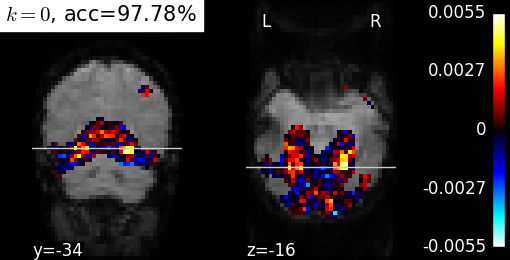
\includegraphics[width=1\linewidth]{figures/haxby_igraphnet_w_0_yz.png}
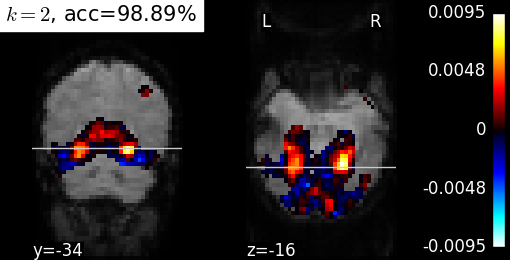
\includegraphics[width=1\linewidth]{figures/haxby_igraphnet_w_2_yz.png}
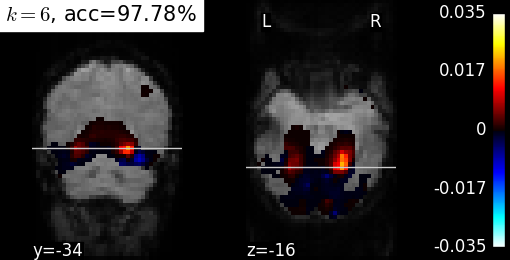
\includegraphics[width=1\linewidth]{figures/haxby_igraphnet_w_6_yz.png}
% 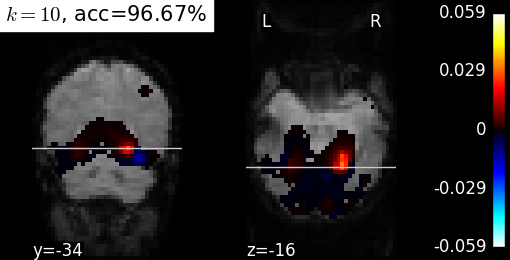
\includegraphics[width=1\linewidth]{figures/haxby_igraphnet_w_10_yz.png}
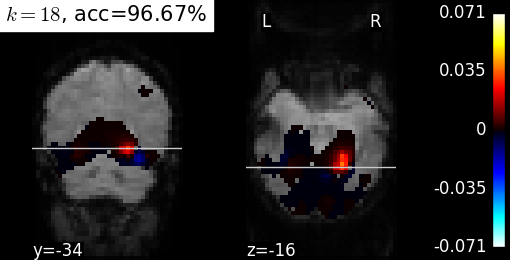
\includegraphics[width=1\linewidth]{figures/haxby_igraphnet_w_18_yz.png}
\caption{Estimated coefficients $\hat{\B{w}}$ on the Face vs House condition
      of the visual recognition dataset \citep{haxby2001}.
Classification accuracies on held-out data are shown in the
legends. We monitor the evolution of the model as a function of the number of iGraphNet iterations $k = 0, 1, 2,\ldots$.
We see that as more and more iterations of iGraphNet are run, the coefficients become more and more spatially denoised and localized (and therefore more
intepretable), without deteriorating of the model accuracy.
% The limit $k \rightarrow \infty$ would correspond to TV-L1 regularization,
% and it is possible that some intermediate finite $k$ strikes an excellent compromise between
}
\vspace{.5cm}
\label{fig:igraphnet}
\end{marginfigure}

\bibliographystyle{plainnat}
\bibliography{bib_all}
